% =============================================================================
% DATA7201 Data Analytics at Scale (2026) — Project Report
% Facebook Ad Library API — third-party advertisers around the 2022 federal
% election.
% =============================================================================

\documentclass[11pt,a4paper]{article}

% ----- packages -------------------------------------------------------------
\usepackage[a4paper, margin=2.5cm]{geometry}
\usepackage[utf8]{inputenc}
\usepackage[T1]{fontenc}
\usepackage{lmodern}
\usepackage{microtype}

\usepackage{graphicx}
\usepackage{booktabs}
\usepackage{tabularx}
\usepackage{caption}
\usepackage{subcaption}
\usepackage{float}

\usepackage{hyperref}
\hypersetup{
  colorlinks=true,
  linkcolor=blue!50!black,
  urlcolor=blue!50!black,
  citecolor=blue!50!black,
}

\usepackage{natbib}
\bibliographystyle{chicago}

\usepackage{listings}
\usepackage{xcolor}
\lstset{
  basicstyle=\ttfamily\footnotesize,
  breaklines=true,
  frame=single,
  showstringspaces=false,
  keywordstyle=\color{blue!50!black},
  commentstyle=\color{green!40!black},
  stringstyle=\color{red!50!black},
}


\title{DATA7201 Data Analytics at Scale - Project Report\\
\small \emph{Examining Non-Government Aligned Election Spending}}
\author{Stewart Fletcher \\ Student Number: s3348393}
\date{\today}


\begin{document}
\maketitle

\begin{abstract}
\noindent This report examines non-government advertisers on the Facebook ad platform around the May 2022 federal election in order to determine the existence of American-style political action committee (PAC) advertisers in Australian elections. \\

Facebook ad data surrounding the election was ingested and preprocessed using PySpark on YARN. A pandas UDF tagged candidate, party, and government advertising via token matching against the Australian Electoral Commission candidate roll. The remaining ads were clustered with Latent Dirichlet Allocation and hand-labelled by category to exclude non-political content. \\

The corpus was then analysed in two ways: a deterministic classifier based upon ad spending before and after the election, and a machine learning classifier using hashtags to create a training dataset for a logistic-regression text classifier. Neither metric alone was sufficient to properly classify advertisers. \\

Third-party advertising was found to be split into a number of distinct patterns, with political advertisers split into two groups: most or all of the ad spending before the election, or constant spending across the period with a pivot to election material before the election. \\

A number of advertisers were subsequently found who matched the PAC-style advertisers seen in the United States, including Climate~200, Smart Voting, GetUp!, ABC Friends, and the Australian Christian Lobby.
\end{abstract}

\newpage
\tableofcontents
\newpage

\section*{Word Count}
\addcontentsline{toc}{section}{Word Count}

Per the assignment specification, the structured abstract, table of contents, captions, tables, and appendices are excluded from the word count. The body word count is \textbf{1{,}646 words}, broken down by section as shown in Table~\ref{tab:wordcount}.

\begin{table}[H]
  \centering
  \begin{tabular}{lr}
    \toprule
    \textbf{Section} & \textbf{Words} \\
    \midrule
    Word Count (this section)                          & 40   \\
    Introduction                                       & 206  \\
    Data ingestion and preparation                     & 215  \\
    Identifying government advertising                 & 126  \\
    Topic clustering via LDA                           & 135  \\
    Temporal analysis: persistence and centroid bands  & 230  \\
    Content analysis: hashtag-supervised classifier    & 275  \\
    Discussion and Conclusions                         & 364  \\
    Section headers                                    & 55   \\
    \midrule
    \textbf{Total}                                     & \textbf{1{,}646} \\
    \bottomrule
  \end{tabular}
  \caption{Word count breakdown produced by \texttt{texcount}.}
  \label{tab:wordcount}
\end{table}

\newpage

\section{Introduction}
Political Action Committees (PACs) are an American campaigning vehicle that raise money for political advertising outside of the existing political structure. Australia does not formally have PACs. Yet independent, third-party advertisers spend millions of dollars on advertising during Australian elections. Identifying these informal Australian ``PACs'' is important for political-advertising transparency, and for finding the boundary between advertisers who are campaigning on specific issues and advertisers who are campaigning on behalf of political parties with private funding.

The Facebook ad platform is attractive for advertisers as it provides access to a large viewer base with minimal effort. Traditional methods such as door-knocking and physical advertising are not required. The Facebook Ad Library is also a convenient data source for finding Australian PAC equivalents. A dataset was provided covering four years of political advertising in Australia, from 2020 to 2024. Although this corpus covered a range of political events, this report focuses on the 2022 Australian federal election.

At approximately 320~GB of JSON files, the dataset cannot easily be analysed on a
conventional workstation. A distributed analytics framework is required. PySpark \citep{zaharia2016apache} was used for its lazy DataFrame API \citep{armbrust2015sparksql}, and Spark MLlib \citep{meng2016mllib} was used for both the unsupervised topic modelling (LDA) and the supervised text classifier (logistic regression).


\section{Dataset Analytics}


\subsection{Data ingestion and preparation}

The data consists of approximately 4{,}500 JSON files containing around 40
million rows spanning February 2020 to March 2024. Each file is a snapshot of
all Australian political advertisements active at that moment, so the same
ad appears in multiple files. Each row represents a single ad with around 25
columns of ad purchaser, Facebook page, creative text, spend, impressions and other fields.
Schema changes occurred in June~2022 and August~2023, with key values becoming sparse thereafter.

A null-fraction analysis was performed to visualise the schema drift.
Automatic schema inference collected the superset of all fields, and the per-column null fraction by month was plotted as a heatmap
(Figure~\ref{fig:null-heatmap}). Columns were then merged to give a consistent schema across the window. Nested struct fields containing string-typed lower and upper bounds were cast to numeric and replaced with their midpoint.

Deduplication was performed by sorting snapshots chronologically per ad ID and tagging each row with an \texttt{ad\_seq\_no} via a \texttt{row\_number()} window operation, where \texttt{1} indicates the most recent snapshot. Filenames used inconsistent date formats and required special handling. The cleaned data was windowed to six months either side of the May 2022 federal election and written as Parquet to HDFS, reducing the corpus from approximately 40~million to 5.7~million rows.

\begin{figure}[H]
  \centering
  \begin{subfigure}[t]{\textwidth}
    \centering
    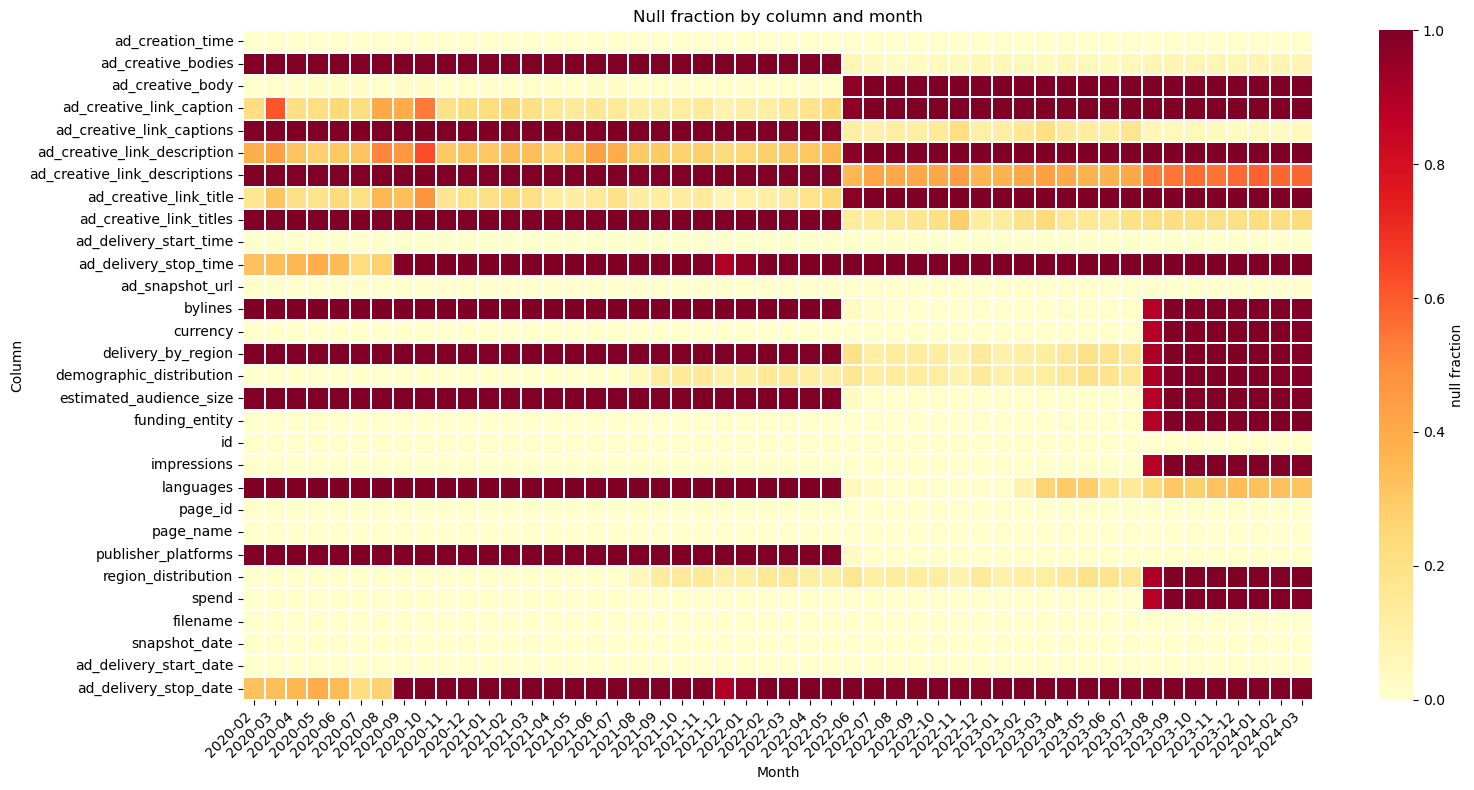
\includegraphics[width=\linewidth]{figures/heatmap_before.png}
    \caption{Before schema correction.}
    \label{fig:null-heatmap-before}
  \end{subfigure}

  \vspace{1em}
  \begin{subfigure}[t]{\textwidth}
    \centering
    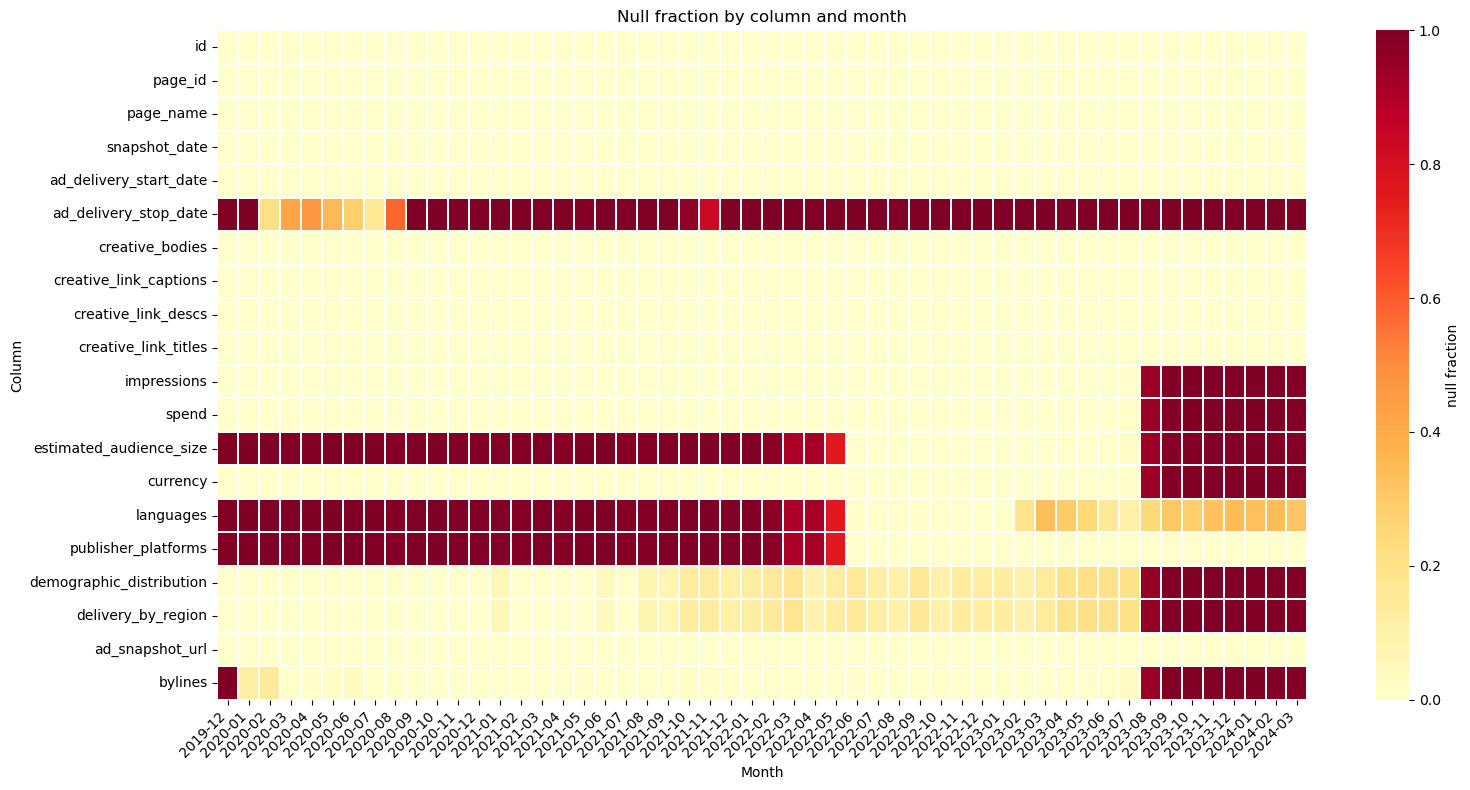
\includegraphics[width=\linewidth]{figures/heatmap_after.png}
    \caption{After schema correction.}
    \label{fig:null-heatmap-after}
  \end{subfigure}
  \caption{Null-fraction heatmaps (column $\times$ month) before and after
  the schema coalesce step. The raw view (top) shows the June 2022
  singular-to-array transition and the August 2023 breakage clearly. The
  cleaned view (bottom) has the duplicate fields merged and a single
  consistent schema across the window. Hot colors show a high percentage of 
  null values for that month/column.}
  \label{fig:null-heatmap}
\end{figure}
\newpage
\subsection{Identifying government advertising}

To focus on third-party organisations the government advertising had to be
removed. This included both political-party advertisements and candidate
advertisements. The 2022 House of Representatives and Senate candidate
rolls were sourced from the Australian Electoral Commission. A straight
join was not effective because page names can be misrepresentative and
the byline can be paid by an aide. Thus a pandas UDF was used to apply three rules in
order with the first match winning, summarised in Table~\ref{tab:match-rules}.

\begin{table}[H]
  \centering
  \begin{tabularx}{\textwidth}{lX}
    \toprule
    \textbf{Rule} & \textbf{Logic and output} \\
    \midrule
    Candidate name
      & The candidate's tokenised name (surname plus first given name)
      is a subset of either the page-name tokens or the byline tokens. \\
    Party byline signature
      & A tokenised party signature from \texttt{aec\_parties.csv} is a
      subset of the byline tokens, e.g.\ $\{$liberal, national$\}
      \rightarrow$ LNP. Signatures are tested longest-first so LNP
      matches before LP. \\
    Government byline signature
      & The byline tokens contain one of $\{$department$\}$,
      $\{$australian, government$\}$, or $\{$australian, electoral,
      commission$\}$. \\
    \bottomrule
  \end{tabularx}
  \caption{Three rules applied by the byline-matching pandas UDF in order,
  first match wins.}
  \label{tab:match-rules}
\end{table}

Every ad was thus tagged according to its nature; ads tagged \texttt{null} (no match against any of the three rules) formed the third-party corpus of interest. The row counts are shown in Table~\ref{tab:match-counts}, with the match-type composition visualised in Figure~\ref{fig:match-type-donuts} and the weekly spending pattern by match-type in Figure~\ref{fig:weekly-spend}.

\begin{table}[H]
  \centering
  \begin{tabular}{lrr}
    \toprule
    \textbf{match\_type} & \textbf{total rows} & \textbf{unique ads}\\
    \midrule
    null         & 4{,}511{,}742 & 105{,}814 \\
    party\_org   & 649{,}857     & 23{,}932  \\
    candidate    & 536{,}232     & 20{,}644  \\
    government   & 98{,}660      & 1{,}188   \\
    \bottomrule
  \end{tabular}
  \caption{Rows and unique ads after government, party, and candidate
  classification.}
  \label{tab:match-counts}
\end{table}

\begin{figure}[H]
  \centering
  \begin{subfigure}[t]{0.49\textwidth}
    \centering
    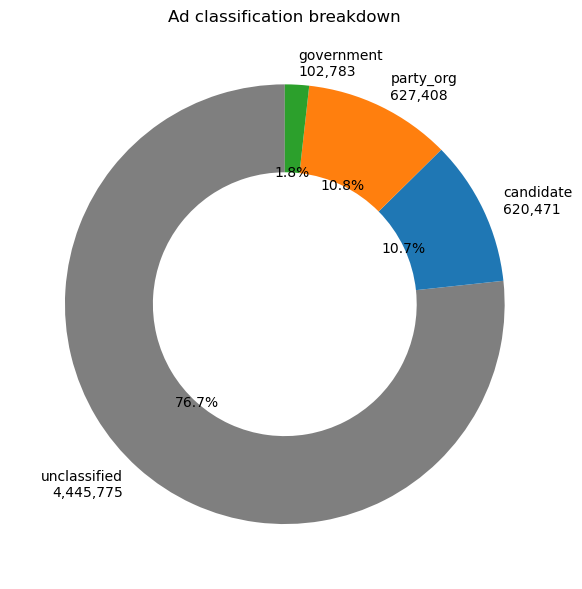
\includegraphics[width=\linewidth]{figures/ad_counts_donut.png}
    \caption{All rows (per snapshot).}
    \label{fig:match-type-donut-rows}
  \end{subfigure}
  \hfill
  \begin{subfigure}[t]{0.49\textwidth}
    \centering
    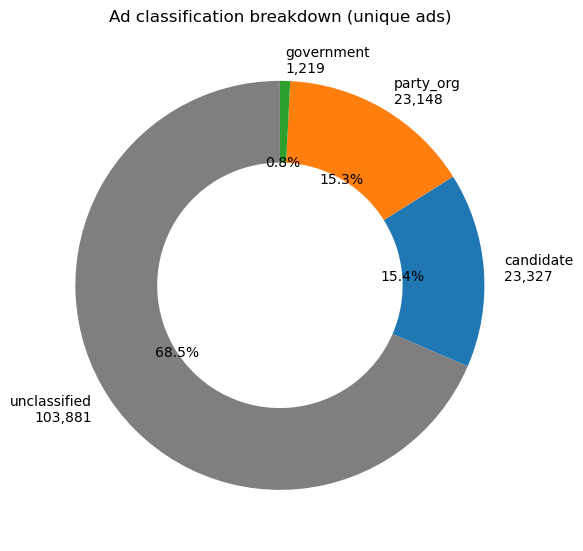
\includegraphics[width=\linewidth]{figures/unqiue_count_donut.png}
    \caption{Unique ads (\texttt{ad\_seq\_no}=1).}
    \label{fig:match-type-donut-unique}
  \end{subfigure}
  \caption{Match-type distribution by total rows (left) and by unique
  ads after deduplication (right). The \texttt{null} bucket dominates by
  both measures and forms the third-party corpus carried forward.}
  \label{fig:match-type-donuts}
\end{figure}

\begin{figure}[H]
  \centering
  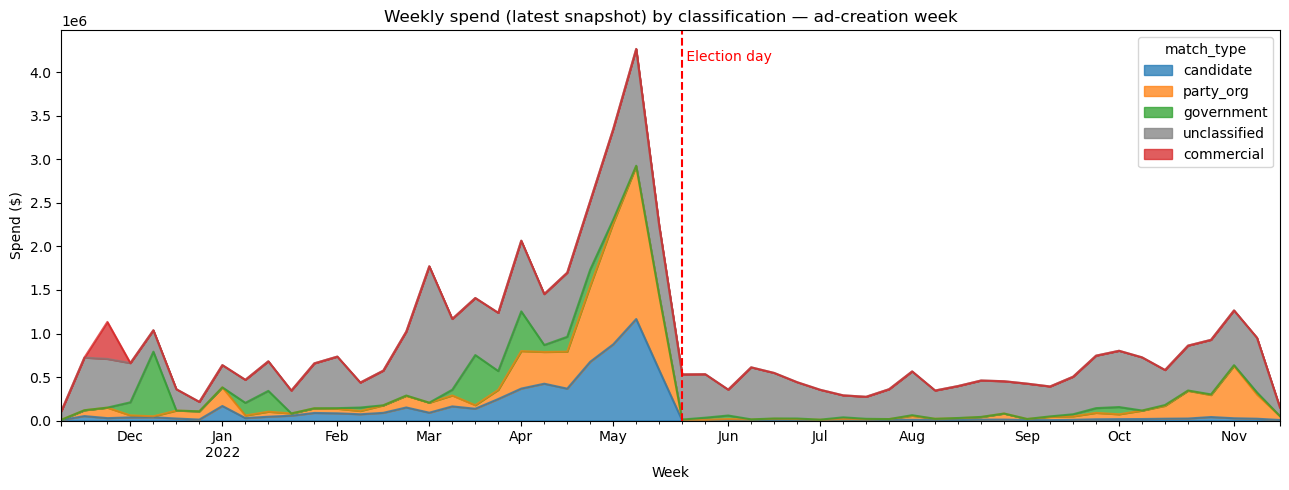
\includegraphics[width=\linewidth]{figures/weekly_spend.png}
  \caption{Weekly spend by match-type across the election window. The
  candidate and party advertising spike around the May 2022 election as
  expected; the \texttt{null} bucket shows a more diffuse pattern, which
  motivates the topic-clustering step in the next subsection.}
  \label{fig:weekly-spend}
\end{figure}

\subsection{Topic clustering via LDA}

The non-government component consisted of a range of topics, not all relevant to the election. Latent Dirichlet Allocation \citep[LDA;][]{blei2003lda} was used to cluster these ads into topic groups based upon the ad text body. After tokenisation, stop-word removal and vectorisation with \texttt{CountVectorizer}, $k=25$ topics were fitted. $k$ was selected by tuning on a subset of the data. The topics were then hand-labelled with the categories \texttt{climate}, \texttt{humanitarian\_rights}, \texttt{political\_advocacy}, \texttt{cost\_of\_living}, and \texttt{mixed}.

Topics without a single coherent theme were tagged as \texttt{mixed} and retained in the corpus, so downstream analysis could choose whether to include them. The result was a corpus of about 95{,}000 advocacy ads, written partitioned by category. The per-topic distribution is shown in Figure~\ref{fig:topics-count}. Of significant interest for this analysis, the largest spending bucket was the non-government \texttt{political\_advocacy} category.

\begin{figure}[H]
  \centering
  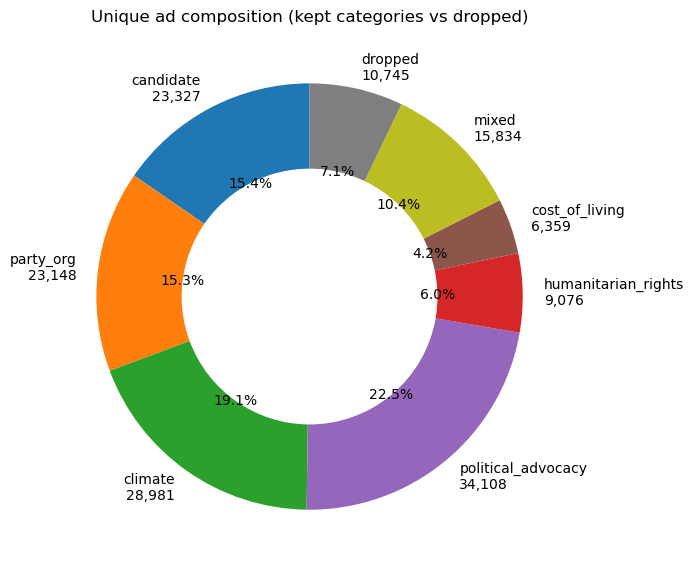
\includegraphics[width=\linewidth]{figures/topics_count.png}
  \caption{Distribution of ads across the 25 LDA topics with the
  hand-assigned categories.}
  \label{fig:topics-count}
\end{figure}

\subsection{Temporal analysis: persistence and centroid bands}

A simple method for identifying ``PAC''-style advertising is to look at spending before and after the election. An advertiser who has a high pre-election spending spike compared to the post-election period is more likely to be focused on the election.

In order to compare advertisers, spending was collated into a weekly time series per advertiser. As the time series was very bursty, a four-week rolling mean was then applied. A hard boundary at the election date was added to prevent bleed over from the pre-election month into the post-election month. The resulting weekly pattern across the non-government corpus is shown in Figure~\ref{fig:non-gov-weekly-spend}.

\begin{figure}[H]
  \centering
  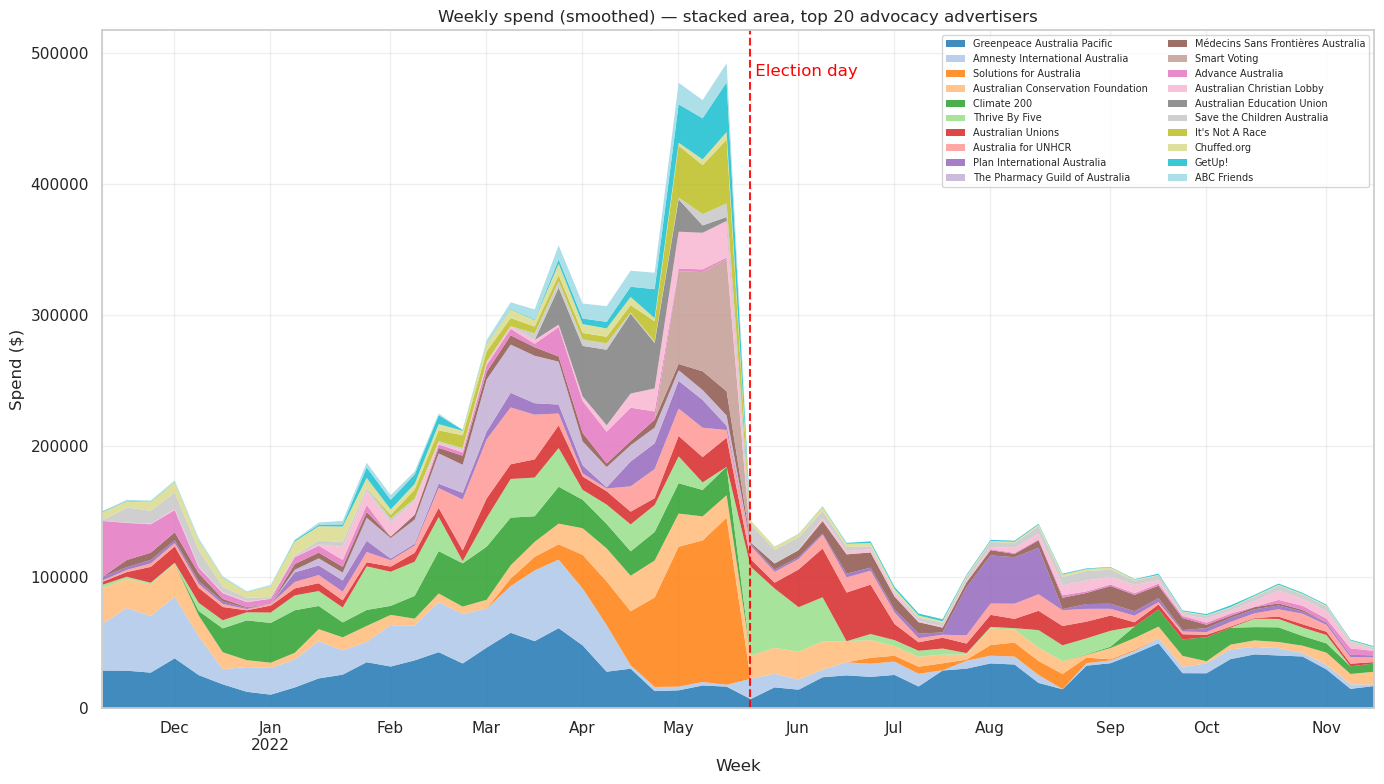
\includegraphics[width=\linewidth]{figures/non-government-weekly_spend.png}
  \caption{Weekly spend across the non-government (advocacy) corpus.
  Spending clusters in the weeks leading up to the May 2022 election and
  drops sharply afterwards.}
  \label{fig:non-gov-weekly-spend}
\end{figure}

A ratio of pre-election spend to post-election spend was calculated and saved as ``persistence''. Investigation of persistence found it was insufficient to identify strong pre-election spenders alone. Early-window spenders received the same weight as near-election spenders, and due to the crossover with the start of the Voice referendum, some political spenders had a late, post-election spend which reduced their ratio.

A second metric was thus developed. ``Centroid'' was the weighted-mean week from election day, where negative values indicate spending before the election and positive values indicate spending after. Centroid was then combined with persistence to identify advertisers who focused their spend in the near pre-election period.

Advertisers were split into four deterministic bands as shown in Table~\ref{tab:bands}. The bands are also plotted on a quadrant in Figure~\ref{fig:quadrant-spend}.

\begin{table}[H]
  \centering
  \begin{tabularx}{\textwidth}{lX}
    \toprule
    \textbf{Band} & \textbf{Rule} \\
    \midrule
    \texttt{election\_only} & persistence $<$ 0.30 and $|$centroid$|$ $\leq$ 16 weeks \\
    \texttt{transitional}   & 0.30 $\leq$ persistence $\leq$ 0.80 \\
    \texttt{ongoing}        & persistence $>$ 0.80 \\
    \texttt{off\_campaign}  & persistence $<$ 0.30 and $|$centroid$|$ $>$ 16 weeks \\
    \bottomrule
  \end{tabularx}
  \caption{Four-band classifier applied to top-20 advertisers.}
  \label{tab:bands}
\end{table}

\begin{figure}[H]
  \centering
  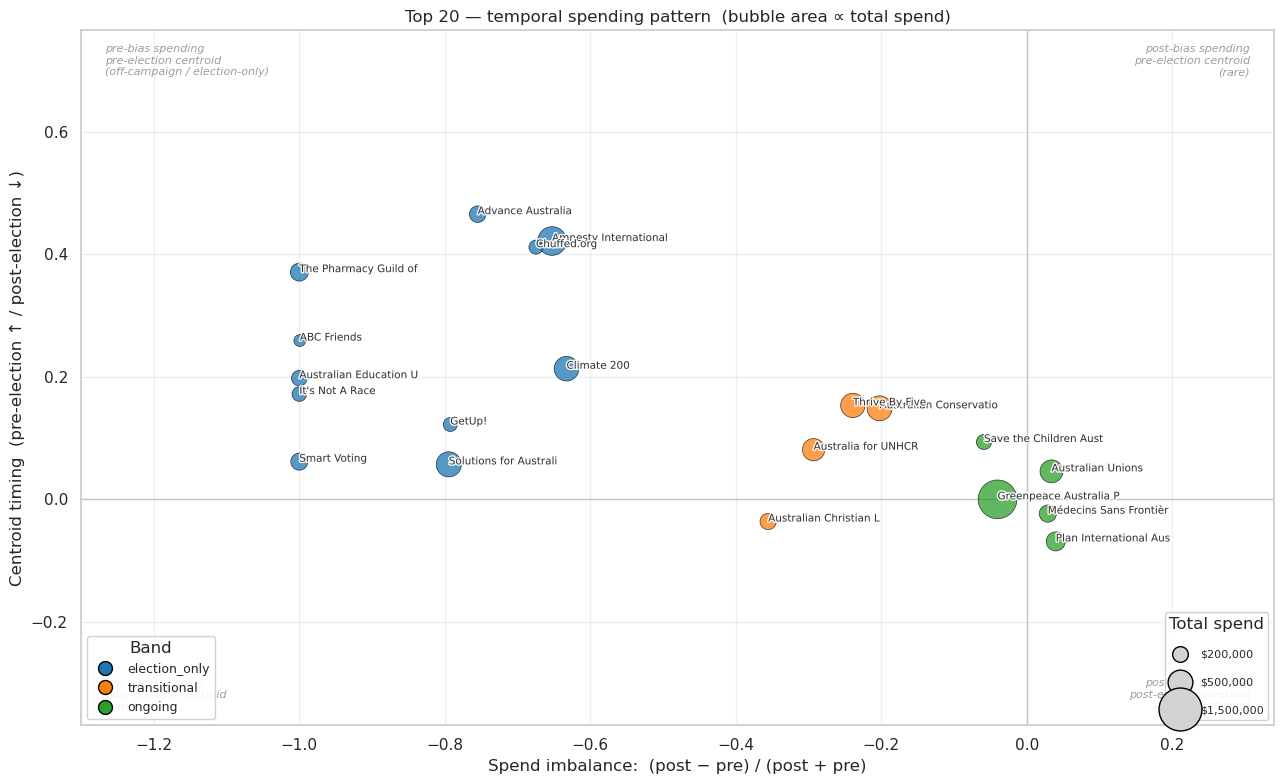
\includegraphics[width=\linewidth]{figures/band_scatter_spend.png}
  \caption{Top 20 non-government advertisers by spend. Low persistance and centroid indicates
  ongoing spend. Larger persistance and a strong negative centroid indicates 
  an advertisiting spend focused on the pre-election period.}
  \label{fig:quadrant-spend}
\end{figure}

\subsection{Content analysis: hashtag-supervised classifier}

Detection based purely upon spending patterns has a number of weaknesses. Firstly, it may identify issue-based advertisers whose spend incidentally peaks before the election. Secondly, the temporal classifier reveals nothing about an advertiser's actual content. Two advertisers with identical spend patterns may be running completely different campaigns. A content-based classifier was added to capture the second case.

Supervised classification requires a training corpus, and after some experimentation hashtags proved a reliable way to extract one. About 210 political hashtags (e.g.\ \texttt{\#federalelection}, \texttt{\#morrisonmustgo}) were drawn from the \texttt{election\_only} category and about 286 non-political hashtags (e.g.\ \texttt{\#breakfreefromplastic}) from the \texttt{ongoing} category, then hand-curated. Labels were assigned as:

\begin{itemize}
  \item Positive: at least one political hashtag, no non-political hashtag.
  \item Negative: at least one non-political hashtag, no political hashtag.
  \item Ambiguous ads excluded from training but scored at inference.
\end{itemize}

Hashtags were stripped from the text prior to vectorisation so the model learned from the body. A logistic regression classifier, a standard approach for high-dimensional bag-of-words text classification \citep{manning2008iir}, was trained on 2{,}599 positive ads from 259 bylines and 5{,}262 negative ads from 303 bylines.

Held-out test AUC was 0.97 (91\% precision, 89\% recall on the positive class). Leave-one-advertiser-out validation was run with a recall of 0.61, suggesting more advanced methods could improve coverage. Inspection of high-scoring no-hashtag ads confirmed the model caught political content the deterministic classification missed, including local-council and state-election candidates running outside the federal-election window.

Per-advertiser scores were aggregated as the mean \texttt{election\_prob} across each advertiser's ads in the 4-week pre-election window. This \texttt{mean\_prob\_pre} metric was then exported for the combined PAC analysis in Section 3. Figure~\ref{fig:content-bar} shows this score across the top-20 spenders.

\begin{figure}[H]
  \centering
  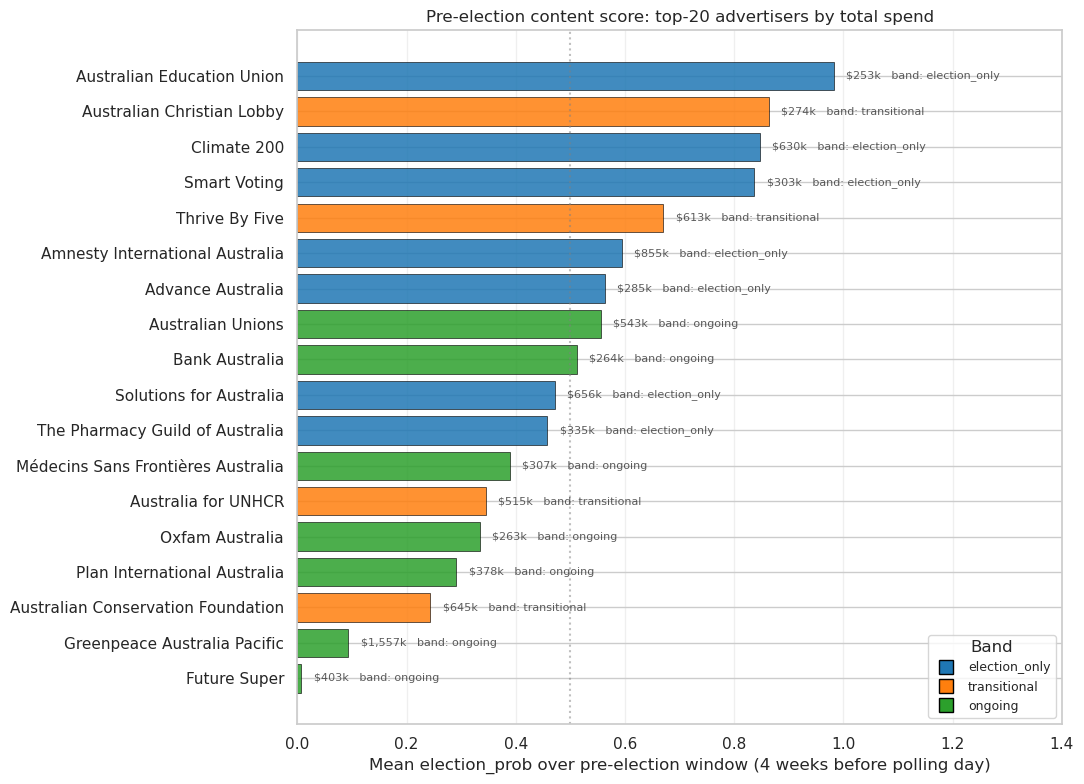
\includegraphics[width=\linewidth]{figures/top_election_classified_in_preelection_spend_band.png}
  \caption{Mean \texttt{election\_prob} over the 4-week pre-election window
  for the top-20 advocacy advertisers by spend, coloured by temporal
  band. Bars longer than 0.5 indicate advertisers whose pre-election
  content reads as predominantly election-themed by the classifier.}
  \label{fig:content-bar}
\end{figure}

\section{Discussion and Conclusions}

Classifying PAC-style advertisers proved more challenging than anticipated. The temporal classifier alone tended to confuse ongoing-issue advocates such as Greenpeace and the Australian Unions with election-window spenders, while the content classifier alone picked up local-council and state-election candidates outside the federal window. Combining the two as a quadrant filter (\texttt{ec\_index > 0.5} and \texttt{mean\_prob\_pre > 0.5}, excluding the \texttt{ongoing} band) produced a reasonable list. More advanced methods, such as transformer-based text models, may potentially improve the result.

\begin{figure}[H]
  \centering
  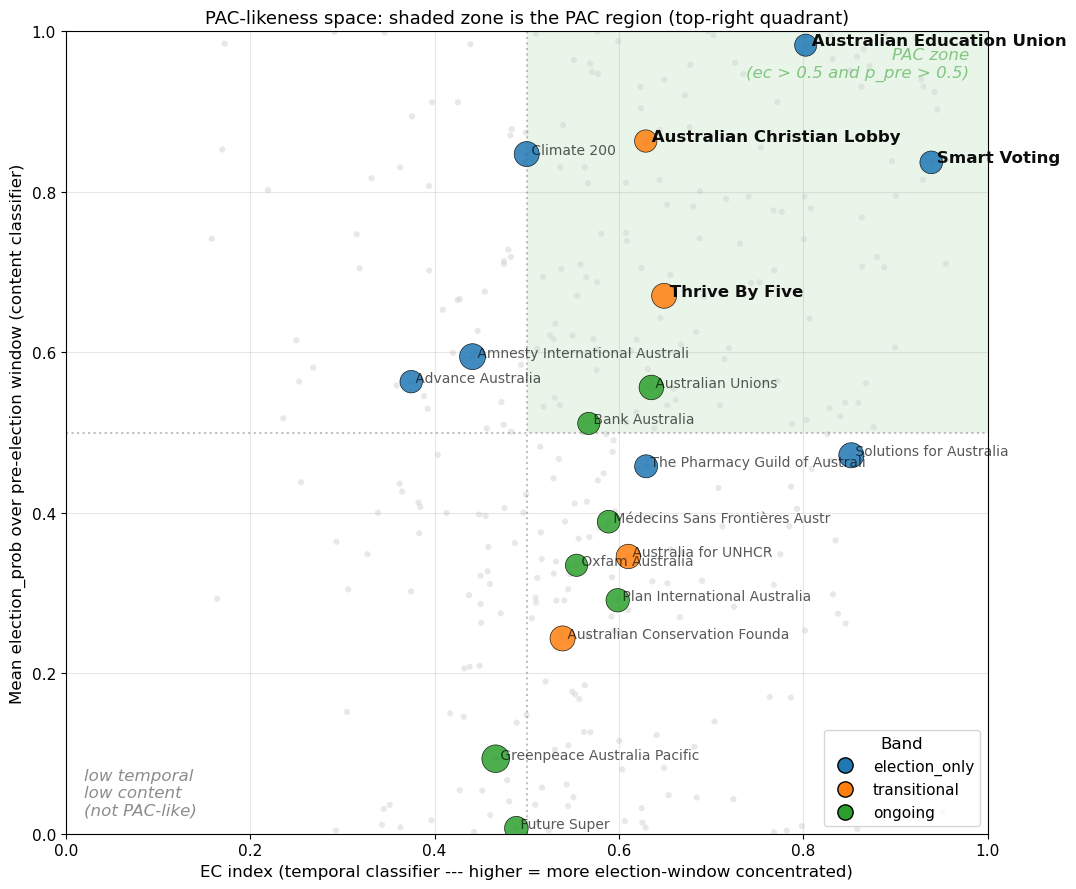
\includegraphics[width=0.85\linewidth]{figures/pac_likeness_scatter.png}
  \caption{Combined PAC-likeness scatter: temporal classifier (\texttt{ec\_index}, x-axis) against content classifier (\texttt{mean\_prob\_pre}, y-axis) for the top-20 advocacy advertisers. The shaded top-right quadrant is the PAC region. Greenpeace sits in the bottom-left despite the largest bubble (\$1.5M).}
  \label{fig:pac-scatter}
\end{figure}

Nevertheless several PAC-style advertisers were identified. These included Smart Voting, the Australian Education Union, Thrive By Five, the Australian Christian Lobby, GetUp!, ABC Friends, and It's Not A Race. Inspection of the top ad titles for each (Table~\ref{tab:top-pacs}) confirmed the classification. All of these advertisers combined a pre-election spend concentration with content that was explicitly partisan or directed at a specific policy outcome.

\begin{table}[H]
  \centering
  \small
  \begin{tabular}{lll}
    \toprule
    \textbf{Advertiser} & \textbf{Band} & \textbf{Top ad title} \\
    \midrule
    Smart Voting               & election\_only & ``Since the Coalition took power, prices have skyrocketed.'' \\
    Australian Education Union & election\_only & ``Properly fund public schools.'' \\
    Thrive By Five             & transitional   & ``Let's make early learning and childcare fair for families.'' \\
    Australian Christian Lobby & transitional   & ``Sign the petition to defend Christian schools.'' \\
    It's Not A Race            & election\_only & ``Government should be about setting the right priorities.'' \\
    GetUp!                     & election\_only & ``Want climate leadership? Vote for it!'' \\
    ABC Friends                & election\_only & ``Save our ABC.'' \\
    \bottomrule
  \end{tabular}
  \caption{Top PAC-style advertisers identified by the combined quadrant filter, with their highest-spend ad title. All combine pre-election spend concentration with explicit issue or party-directional messaging.}
  \label{tab:top-pacs}
\end{table}

The major outlier was Greenpeace. At \$1.5M it was the largest non-government advertiser in the dataset. However it satisfied none of the PAC criteria, with a fairly constant spend curve and a mean pre-election content score of 0.09. Inspection of the top Greenpeace ads found that the May 2022 campaign was focused on Woodside Petroleum, not the federal election. Thus a high advertising spend during an election window does not, on its own, indicate PAC-style behaviour.

Despite the limitations of the classifiers a reasonably confident list of Australian PAC-style advertisers can be identified from this dataset. Australia does not have formal PACs, but their informal equivalents do operate around federal elections. As discussed in the introduction, the boundary between issue advocacy and party-aligned third-party campaigning is one that traditional campaign-finance disclosure cannot easily examine. The combination of the Facebook Ad Library and the analytical methods demonstrated here may allow this boundary to be examined at a scale not previously available.

The scale of the dataset meant that the analysis was only practical using a distributed framework. The 40-million-row, 320~GB JSON corpus could not have been deduplicated, clustered with LDA, or joined against the candidate roll on a conventional workstation in any reasonable time. Distributed storage, lazy DataFrame evaluation, and the Spark MLlib library were all used to make the full analysis viable.

\bibliography{references}

% =============================================================================
\appendix
\section{Use of Generative AI}
% =============================================================================
Claude (Anthropic; the \texttt{claude-opus-4-7} model accessed via the
Claude Code CLI between April and May 2026) was used as a proofreading
and editing assistant and as a coding agent during the preparation of
this project. Its use is described below.

\begin{itemize}
  \item \textbf{Writing.} The text of this report was written by the
  author. Claude's role in the writing was limited to proofreading and
  copy-editing: identifying typographical and grammatical errors,
  suggesting minor wording refinements, and flagging inconsistencies
  between paragraphs. All substantive content --- the framing of the
  problem, the analytical argument, the choice of which findings to
  highlight, and the structure and narrative of the report --- was
  authored and decided by the student.
  \item \textbf{Plotting.} Claude was primarily used as a teaching aide,
  using an interactive session to query issues rather than a search engine. 
  Claude directly assisted with parts of the matplotlib
  visualisation code (donut charts, stacked-area plots, small multiples,
  and the quadrant scatter plots in notebooks 02, 04 and 05). The
  PySpark and pandas analysis pipeline was written by the author. All
  visualisation code generated with Claude's assistance was reviewed,
  tested, and integrated by the author.
\end{itemize}

The author retained responsibility for all analytical, code, and
editorial decisions throughout, and verified the correctness of all
code, numerical results, and claims before they were included in this
report. Full conversation transcripts can be supplied on request.

% =============================================================================
\section{Code}
% =============================================================================
The full analysis pipeline is implemented in six Jupyter notebooks at
\url{https://github.com/<USER>/FB_API} (replace with the actual URL).
Each notebook is self-contained and writes its output as Parquet on HDFS or
as CSV in the repository's \texttt{data/} directory.

\begin{description}
  \item[\texttt{01\_data\_loading.ipynb}] Raw JSON ingestion, schema
  flattening, deduplication, window filtering, write of v1 Parquet.
  \item[\texttt{02\_preprocessing.ipynb}] Candidate, party, and government
  byline matching via pandas UDF; write of v2 Parquet.
  \item[\texttt{03\_topics.ipynb}] LDA topic modelling, $k$ sweep, topic
  inspection, output of \texttt{topic\_terms.csv} for hand-labelling.
  \item[\texttt{04\_topic\_join.ipynb}] Join of hand-labelled topics onto
  v2, filter to political-adjacent residual, write of v3 Parquet.
  \item[\texttt{04b\_hashtag\_analysis.ipynb}] Regex extraction of hashtags
  across v3, count by band, export of \texttt{data/hashtags.csv}.
  \item[\texttt{05\_election\_spenders.ipynb}] Top-20 ranking, weekly
  aggregation, election-boundary smoothing, persistence + centroid
  computation, four-band classification, export of band CSVs and
  visualisations.
  \item[\texttt{06\_election\_content\_classifier.ipynb}] Hashtag-supervised
  logistic-regression text classifier; FP / FN / LOO validation;
  per-advertiser and per-week scoring; pivot-detection table.
\end{description}

Selected code excerpts follow.

\subsection*{Election-boundary smoothing (nb 05)}
\begin{lstlisting}[language=Python]
# Hard smoothing boundary at election day --- pre and post halves
# smoothed independently so cliff-edged advertisers do not bleed forward.
weekly['is_post'] = weekly['week'] >= ELECTION_DATE
weekly['spend_smooth'] = (weekly
    .groupby(['bylines', 'is_post'])['spend']
    .transform(lambda s: s.rolling(window=4, center=True, min_periods=1).mean()))
\end{lstlisting}

\subsection*{Hashtag-supervised labelling (nb 06)}
\begin{lstlisting}[language=Python]
pol_re = r'#(' + '|'.join(re.escape(t) for t in political_hashtags) + r')\b'
non_re = r'#(' + '|'.join(re.escape(t) for t in non_political_hashtags) + r')\b'

v3 = v3.withColumn('has_political_hashtag',     col('raw_text').rlike(pol_re))
v3 = v3.withColumn('has_non_political_hashtag', col('raw_text').rlike(non_re))

# Strip hashtags before vectorising --- model must learn from surrounding prose.
v3 = v3.withColumn('text', regexp_replace(col('raw_text'), r'#\w+', ' '))

labelled = v3.withColumn('label',
    when( col('has_political_hashtag') & ~col('has_non_political_hashtag'), 1.0)
    .when(~col('has_political_hashtag') &  col('has_non_political_hashtag'), 0.0)
    .otherwise(None))
\end{lstlisting}

\end{document}
